\documentclass[11pt]{article}
\usepackage[margin=0.78in]{geometry}
\usepackage[T1]{fontenc}
\usepackage[utf8]{inputenc}
\usepackage{lmodern}
\usepackage{amsmath,amssymb}
\usepackage{graphicx}
\usepackage{hyperref}
\usepackage{caption}
\usepackage{microtype}
\usepackage{booktabs}
\usepackage{xcolor}
\usepackage{titlesec}
\usepackage{enumitem}

\captionsetup{font=small,labelfont=bf}
\setlist[itemize]{leftmargin=1.1em, itemsep=0.2em, topsep=0.35em}
\setlist[enumerate]{leftmargin=1.25em, itemsep=0.2em, topsep=0.35em}
\definecolor{LinkBlue}{HTML}{1F4E79}
\titleformat{\section}{\large\bfseries}{\thesection}{0.5em}{}
\titleformat{\subsection}{\normalsize\bfseries}{\thesubsection}{0.5em}{}
\titleformat{\subsubsection}{\normalsize\bfseries}{\thesubsubsection}{0.5em}{}
\titlespacing*{\section}{0pt}{1.2ex plus .2ex minus .2ex}{0.5ex}
\titlespacing*{\subsection}{0pt}{0.9ex plus .2ex minus .2ex}{0.35ex}
\titlespacing*{\subsubsection}{0pt}{0.8ex plus .2ex minus .2ex}{0.25ex}
\hypersetup{colorlinks=true,linkcolor=black,citecolor=black,urlcolor=LinkBlue}
\setlength{\textfloatsep}{12pt plus 2pt minus 3pt}
\setlength{\floatsep}{10pt plus 2pt minus 2pt}
\setlength{\intextsep}{10pt plus 2pt minus 2pt}
\raggedbottom

\newcommand{\appendixsnapshot}{%
{\small
\setlength{\tabcolsep}{6pt}
\renewcommand{\arraystretch}{1.08}
\sloppy
% Auto-generated paper appendix fragment.
\subsection*{Appendix Snapshot}
This appendix summarizes the pooled OpenAI GPT and Anthropic Claude benchmark over 6912 scored responses. The full machine-generated statistics remain available separately in \texttt{appendix\_snapshot\_full.tex}.
The pooled fit yields $\alpha=3.262$ with 95\% interval $[2.959, 3.558]$ and $\beta=0.092$ with interval $[-0.279, 0.460]$.

\subsubsection*{Top-Line Summary}
\begin{center}
\begin{tabular}{lr}
\toprule
Metric & Value \\
\midrule
Usable evaluations & 6912 \\
Mean $d_{phys}$ & 0.408 \\
Median $d_{phys}$ & 0.302 \\
Exact-correct rate & 0.345 \\
$d_{phys} \ge 0.5$ rate & 0.403 \\
Full-error rate & 0.274 \\
Best model & Claude Opus 4.1 \\
Weakest model & GPT-4o mini \\
\bottomrule
\end{tabular}
\end{center}

\subsubsection*{Model Ranking}
\begin{center}
\begin{tabular}{lrrrr}
\toprule
Model & Mean & 95\% CI & Exact & Full \\
\midrule
Claude Opus 4.1 & 0.138 & [0.116, 0.160] & 0.582 & 0.082 \\
GPT-5.4 & 0.329 & [0.301, 0.357] & 0.430 & 0.195 \\
GPT-5.2 & 0.368 & [0.338, 0.397] & 0.380 & 0.249 \\
GPT-5.4 mini & 0.394 & [0.364, 0.424] & 0.372 & 0.267 \\
GPT-4.1 & 0.442 & [0.412, 0.471] & 0.311 & 0.293 \\
Claude Sonnet 4 & 0.450 & [0.419, 0.481] & 0.305 & 0.332 \\
GPT-4.1 mini & 0.478 & [0.449, 0.507] & 0.285 & 0.311 \\
GPT-5.1 & 0.501 & [0.472, 0.531] & 0.260 & 0.355 \\
GPT-4o mini & 0.570 & [0.543, 0.598] & 0.177 & 0.378 \\
\bottomrule
\end{tabular}
\end{center}

\subsubsection*{Depth and Category Breakdown}
\noindent\begin{minipage}[t]{0.42\linewidth}
\centering
\textbf{By depth}\\[0.25em]
\begin{tabular}{rrrr}
\toprule
Depth & Mean & Exact & Full \\
\midrule
1 & 0.403 & 0.349 & 0.275 \\
2 & 0.415 & 0.340 & 0.275 \\
4 & 0.405 & 0.345 & 0.271 \\
\bottomrule
\end{tabular}
\end{minipage}\hfill
\begin{minipage}[t]{0.54\linewidth}
\centering
\textbf{By category}\\[0.25em]
\begin{tabular}{lrrr}
\toprule
Category & Mean & Exact & Full \\
\midrule
Circuit & 0.657 & 0.213 & 0.476 \\
Measurement & 0.520 & 0.284 & 0.417 \\
Operator & 0.258 & 0.078 & 0.006 \\
Entanglement & 0.196 & 0.804 & 0.196 \\
\bottomrule
\end{tabular}
\end{minipage}

\subsubsection*{Model-by-Category Means}
\begin{center}
\begin{tabular}{lrrrr}
\toprule
Model & Circuit & Measurement & Operator & Entanglement \\
\midrule
Claude Opus 4.1 & 0.367 & 0.068 & 0.117 & 0.000 \\
GPT-5.4 & 0.592 & 0.509 & 0.215 & 0.000 \\
GPT-5.2 & 0.659 & 0.587 & 0.224 & 0.000 \\
GPT-5.4 mini & 0.721 & 0.586 & 0.270 & 0.000 \\
GPT-4.1 & 0.697 & 0.552 & 0.283 & 0.234 \\
Claude Sonnet 4 & 0.658 & 0.432 & 0.258 & 0.453 \\
GPT-4.1 mini & 0.728 & 0.635 & 0.308 & 0.240 \\
GPT-5.1 & 0.707 & 0.602 & 0.302 & 0.396 \\
GPT-4o mini & 0.786 & 0.711 & 0.347 & 0.438 \\
\bottomrule
\end{tabular}
\end{center}

\subsubsection*{Anthropic Repair Ablation}
After fixing output extraction to score the final machine-readable literal even when it is preceded by explanatory text, we ran a separate 32-task Claude repair ablation using Claude Sonnet 4 and Claude Opus 4.1 at depth 4 with a five-minute per-prompt budget.

\begin{center}
\begin{tabular}{lrrr}
\toprule
Mode & Solve rate & Mean solve time & Median solve time \\
\midrule
One-shot & 0.594 & 6.114 s & 6.383 s \\
Self-retry & 0.812 & 7.506 s & 6.806 s \\
Verifier feedback & 0.938 & 11.258 s & 7.114 s \\
\bottomrule
\end{tabular}
\end{center}

\noindent Category solve rates under the same Claude repair ablation were:
\begin{center}
\begin{tabular}{lccc}
\toprule
Category & One-shot & Self-retry & Verifier feedback \\
\midrule
Circuit & 0.625 & 0.625 & 0.875 \\
Measurement & 0.625 & 0.875 & 0.875 \\
Operator & 0.500 & 0.750 & 1.000 \\
Entanglement & 0.625 & 1.000 & 1.000 \\
\bottomrule
\end{tabular}
\end{center}

\noindent By model, Claude Opus 4.1 solved all 32 subset prompts in every repair mode, while Claude Sonnet 4 improved from 0.188 one-shot solve rate to 0.625 with self-retry and 0.875 with verifier feedback.

}%
}

\title{QuantumPhysEval: Measuring Quantum Hallucinations in LLMs}
\author{Anonymous Authors}
\date{}

\begin{document}
\maketitle

\begin{abstract}
This paper presents QuantumPhysEval, a benchmark developed to measure whether large language models produce physically inconsistent yet superficially plausible answers on elementary quantum-mechanical tasks. QuantumPhysEval evaluates model behavior in four task families central to introductory quantum reasoning: circuit evolution, operator composition, measurement prediction, and entanglement classification. Because the benchmark is built from analytically generated small-system quantum problems, it supports exact self-generated ground truth and fully automated scoring with bounded normalized physics-error metrics. Through a case study involving seven OpenAI GPT-family models and two Anthropic Claude-family models across three prompted reasoning-depth settings, QuantumPhysEval identifies clear reliability gaps and offers practical insight into where those models fail. In the pooled 2-qubit analysis of 6{,}912 evaluations, benchmark error decreases strongly with a model-size proxy, with fitted exponent $\alpha=3.262$ and bootstrap 95\% interval $[2.959, 3.558]$, while prompted reasoning depth shows only a weak effect with $\beta=0.092$ and interval $[-0.279, 0.460]$. In a matched 4-qubit stress test over the same model sets, mean error rises from 0.408 to 0.533, with the largest degradations in circuit evolution ($+0.185$) and measurement prediction ($+0.188$). A separate 64-task OpenAI repair ablation shows that one-shot solving reaches 0.422 solved fraction, blind self-retry reaches 0.609, and verifier-guided retry reaches 0.688, with nearly all gains saturating within the first 30 seconds. After adding robust final-literal extraction for mixed prose and code-block outputs, a matched 32-task Claude repair ablation yields 0.594 one-shot solve rate, 0.813 self-retry, and 0.938 verifier-feedback solve rate. The largest residual risks in the pooled benchmark remain concentrated in circuit evolution and measurement prediction, indicating that exact quantum dynamics remain difficult even for stronger recent models.
\end{abstract}

\section{Introduction}
Large Language Models (LLMs) have shown strong performance on many reasoning and coding tasks, but there are still relatively few benchmarks designed to measure whether their outputs remain faithful to exact scientific structure. In quantum information settings, this matters because correct answers must satisfy sharply defined physical constraints such as normalization, unitarity, linear state evolution, and the Born rule. An answer can therefore look polished and plausible while still being physically wrong.

In this work, we identify one major reliability risk for language models in this domain: \emph{quantum hallucination}, which we define as a model output that is syntactically plausible but inconsistent with exact quantum-mechanical ground truth or with basic physical constraints. To measure this risk, we develop QuantumPhysEval, an evaluation suite intended to integrate directly into model testing workflows in the same way that safety and robustness benchmarks are used in other domains.

\subsection{QuantumPhysEval Approach}
QuantumPhysEval's overall approach is straightforward. First, we construct benchmark prompts from analytically generated quantum tasks so that exact targets are known by construction. Second, we score model outputs using bounded physics-grounded error metrics rather than subjective grading. Third, we apply the resulting benchmark to multiple model families and prompted depth settings in order to understand which kinds of quantum tasks remain difficult and whether stronger models reduce those errors. The primary case study uses exact 2-qubit tasks, and a matched 4-qubit stress test measures how reliability changes as the state space expands.

This benchmark is designed to be useful in practice. Because test generation, target generation, and evaluation are automated, the suite can be rerun easily as models improve. Because it uses exact small-system simulation, every failure corresponds to a real physical inconsistency rather than a matter of interpretation.

\subsection{Main Contributions}
Overall, QuantumPhysEval makes the following contributions:
\begin{itemize}
\item \textbf{Exactness}: every test case has an exact self-generated quantum target derived analytically inside the harness.
\item \textbf{Breadth}: the benchmark covers four distinct quantum reasoning families: circuit evolution, operator composition, measurement prediction, and entanglement classification.
\item \textbf{Automation}: test generation, model querying, parsing, scoring, and scaling-law fitting are fully automated.
\item \textbf{Actionability}: in a pooled OpenAI GPT and Anthropic Claude case study, the benchmark identifies concrete reliability gaps and isolates the task families that drive them.
\end{itemize}

\subsection{The structure of this paper}
The rest of the paper is organized as follows. First, we describe QuantumPhysEval's benchmark construction and scoring methodology. Next, we describe the case study protocol used to evaluate pooled OpenAI GPT and Anthropic Claude models. We then present top-level results, category-level findings, and ablations. Finally, we discuss limitations and conclude.

\section{Benchmark Construction}
\begin{figure}[tbp]
\centering
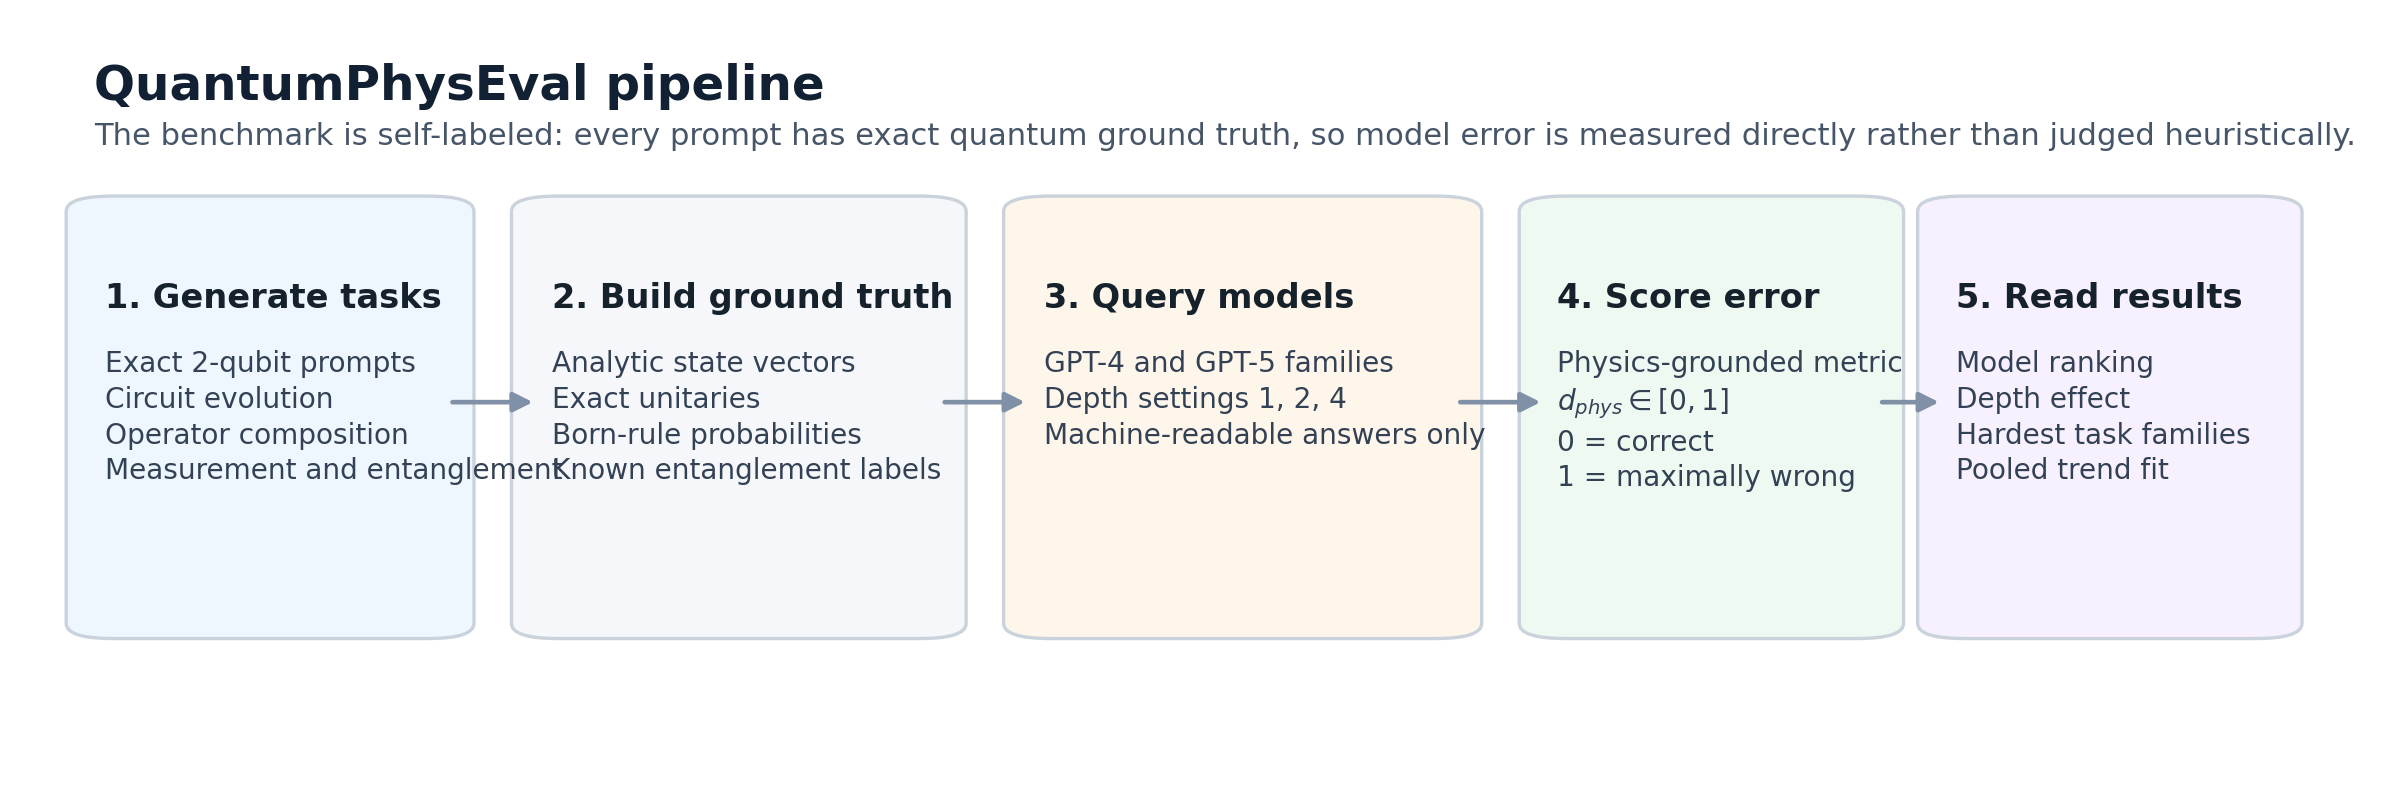
\includegraphics[width=0.98\linewidth]{../artifacts/figures/quantumphys_eval_overview.png}
\caption{QuantumPhysEval benchmark overview. The pipeline is fully automated: exact small-system tasks are generated analytically, exact targets are computed by construction, model outputs are scored with a bounded physics-grounded error metric, and pooled trends are analyzed across model families and depth settings. The main case study uses 2-qubit tasks, and a matched 4-qubit stress test measures difficulty growth.}
\label{fig:overview}
\end{figure}

QuantumPhysEval contains four benchmark families:
\begin{itemize}
\item \textbf{Circuit evolution}: generate the final quantum state after a sampled gate sequence.
\item \textbf{Operator composition}: generate the exact one-qubit unitary corresponding to a sampled gate sequence.
\item \textbf{Measurement prediction}: generate the exact post-circuit measurement probabilities.
\item \textbf{Entanglement classification}: decide whether a provided two-qubit state is entangled.
\end{itemize}

\subsection{Constructing test cases}
All benchmark instances are generated analytically inside the evaluation harness. The gate library consists of single-qubit gates $\{I,H,X,Y,Z,S,T\}$ and two-qubit gates built from $\mathrm{CNOT}$ and $\mathrm{CZ}$. For circuit evolution and measurement prediction, the benchmark samples initial states and gate sequences and then computes exact outcomes. For operator composition, it samples one-qubit gate sequences and asks the model to return the corresponding unitary. For entanglement classification, it evaluates analytically specified product and entangled states. The primary pooled benchmark uses exact 2-qubit tasks; the matched stress test extends circuit evolution, measurement prediction, and entanglement classification to 4 qubits while keeping operator composition as a fixed one-qubit control task.

Each run contains 64 prompts per benchmark family, yielding 256 unique prompts per run. Because the benchmark is generated from exact quantum primitives rather than mined from free-form text, the task distribution is controlled and reproducible.

\subsection{Generating exact ground truth}
Ground truth is produced directly from quantum mechanics rather than external annotation. States and operators are computed by explicit matrix multiplication. Measurement targets are derived from exact Born-rule probabilities. Entanglement labels are attached by construction. This allows the benchmark to avoid noisy labels and to support exact automated evaluation. It also makes matched difficulty expansions possible, since the same harness can be rerun at larger qubit counts with exact targets.

\section{Methods}
Each model response is parsed into a structured object and scored with a bounded physics-grounded error metric $d_{phys}\in[0,1]$, where 0 indicates a correct response and 1 indicates a maximally bad or unparseable response under the benchmark metric.

\subsection{Scoring state, operator, probability, and boolean outputs}
For circuit-evolution tasks, the predicted state is normalized, aligned up to global phase, and compared to the exact target using a combination of normalization penalty and one minus fidelity. For measurement tasks, negative values are clipped to zero, the output is renormalized, and the score combines total-variation distance with a normalization penalty. For operator-composition tasks, the score averages a unitarity penalty with a target-mismatch penalty based on normalized Frobenius norms. For entanglement classification, the score is 0 for an exact match and 1 otherwise.

These metrics are intentionally simple. The goal is not to model every nuance of how a human instructor would grade a quantum mechanics homework answer; the goal is to determine whether the model returned an object that is physically consistent with the exact target. To avoid confounding provider-specific formatting style with scientific correctness, the parser first attempts to read the full response as a literal and then falls back to extracting the final bracketed literal or boolean token when a model returns the answer after explanatory text or inside a code block.

\subsection{Case study protocol}
To study benchmark behavior in practice, we apply QuantumPhysEval to three completed 2-qubit runs. The first evaluates \texttt{gpt-4o-mini}, \texttt{gpt-4.1-mini}, and \texttt{gpt-4.1}. The second evaluates \texttt{gpt-5.1}, \texttt{gpt-5.2}, \texttt{gpt-5.4-mini}, and \texttt{gpt-5.4}. The third evaluates Claude Sonnet 4 and Claude Opus 4.1. Each model is tested at prompted reasoning-depth settings $D\in\{1,2,4\}$ with temperature fixed at 0.0. The system prompt enforces machine-readable answers only, and the user prompt requests the specified number of internal reasoning steps while returning only the final answer.

Across all three runs, the pooled 2-qubit evaluation contains 6{,}912 scored responses. To summarize aggregate scaling behavior, we fit
\[
\mathbb{E}[d_{phys}] = k S^{-\alpha} D^{\beta},
\]
using a model-size proxy $S$ and log-linear least squares, with 2{,}000 bootstrap resamples for uncertainty estimation.

We then run a matched 4-qubit stress test on the same GPT and Claude model sets. This stress test adds another 6{,}912 scored responses and keeps the category schema fixed so that differences can be compared directly. Circuit evolution, measurement prediction, and entanglement classification are upgraded to 4 qubits, while operator composition remains a 1-qubit control slice to separate genuine state-space effects from generic output-format effects.

\subsection{Time-budget repair ablation}
We also run a separate repair ablation designed to test whether the hardest failures are recoverable with additional interaction time. This ablation uses a strong-model subset consisting of \texttt{gpt-4.1}, \texttt{gpt-5.2}, \texttt{gpt-5.4-mini}, and \texttt{gpt-5.4}; depth 4 only; temperature 0.2; and four prompts per benchmark family, for 64 tasks total. Each prompt receives a five-minute wall-clock budget and is evaluated under three modes: \emph{one-shot} (no retry), \emph{self-retry} (the model takes another pass without being told whether the prior answer was wrong), and \emph{verifier feedback} (the model is told only that the prior answer was incorrect against exact ground truth).

For this ablation we report solved fraction by deadline (pass@30s, pass@60s, pass@120s, pass@300s), mean and median time-to-correctness among solved prompts, and category- and model-level solved fractions. The goal is to distinguish failures that are fixable with iterative inference from failures that persist even under repeated repair attempts.

\section{Results}
\subsection{Top-level findings}
The pooled mean normalized error is 0.408, with median 0.302. Exact-correct outputs occur on 34.5\% of samples, while 27.4\% of samples are effectively full-error failures. QuantumPhysEval is therefore measuring a substantial reliability gap rather than just small calibration drift.

As shown in Table~\ref{tab:model-ranking}, the strongest model in the pooled case study is Claude Opus 4.1 and the weakest is \texttt{gpt-4o-mini}. The ordering is not perfectly monotone with the manually assigned size proxy, but the overall trend is clear: more capable models reduce physics-grounded benchmark error.

\begin{table}[t]
\centering
\caption{Mean normalized physics error by model in the pooled case study. Lower is better.}
\label{tab:model-ranking}
\begin{tabular}{lr}
\toprule
Model & Mean $d_{phys}$ \\
\midrule
Claude Opus 4.1 & 0.138 \\
\texttt{gpt-5.4} & 0.329 \\
\texttt{gpt-5.2} & 0.368 \\
\texttt{gpt-5.4-mini} & 0.394 \\
\texttt{gpt-4.1} & 0.442 \\
Claude Sonnet 4 & 0.450 \\
\texttt{gpt-4.1-mini} & 0.478 \\
\texttt{gpt-5.1} & 0.501 \\
\texttt{gpt-4o-mini} & 0.570 \\
\bottomrule
\end{tabular}
\end{table}

The following theses emerged from the pooled benchmark results:
\begin{enumerate}
\item All studied models exhibit quantum hallucinations at non-trivial rates.
\item More capable models reduce those errors, but do not eliminate them.
\item Prompted reasoning depth has only a weak effect relative to model capability.
\item The largest failures are concentrated in exact quantum dynamics tasks.
\end{enumerate}

\begin{figure}[tbp]
\centering
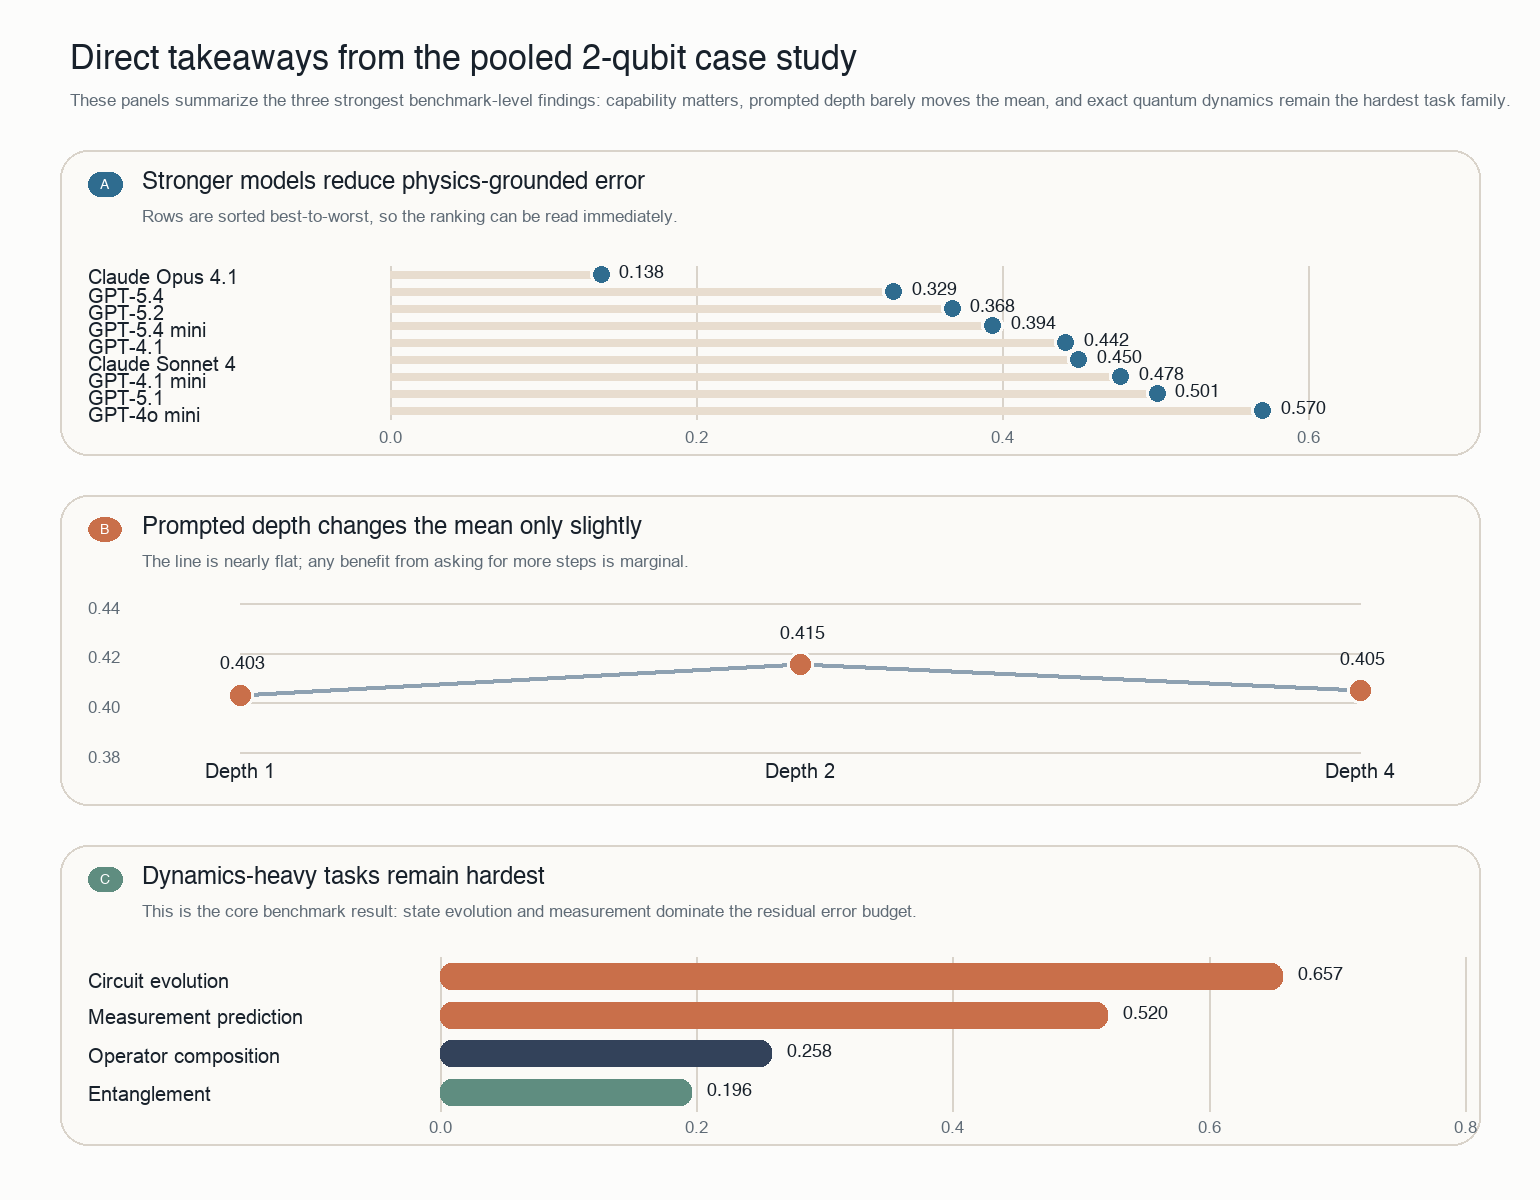
\includegraphics[width=0.98\linewidth]{../artifacts/figures/combined_quantum_takeaways.png}
\caption{Direct takeaways from the pooled OpenAI GPT and Anthropic Claude case study. Left: stronger models reduce physics-grounded error. Middle: more prompted reasoning depth changes the result only slightly. Right: the hardest residual failures remain circuit evolution and measurement prediction.}
\label{fig:takeaways}
\end{figure}

\subsection{Scaling behavior}
The strongest quantitative pattern in the pooled analysis is the size effect. Fitting the pooled data yields
\[
\alpha = 3.262 \quad \text{with bootstrap 95\% CI } [2.959, 3.558].
\]
Under the current proxy assignment, this supports a strong decrease in benchmark error with model capability or scale.

The prompted reasoning-depth effect is much weaker:
\[
\beta = 0.092 \quad \text{with bootstrap 95\% CI } [-0.279, 0.460].
\]
Average error at depth 4 is 0.405, compared with 0.403 at depth 1 and 0.415 at depth 2. We therefore do not find robust evidence that increasing the prompted depth condition alone materially improves benchmark performance.

\subsection{Benchmark-family findings}
Benchmark-family differences are pronounced. In the pooled run, category means are:
\begin{itemize}
\item \textbf{Circuit evolution}: 0.657
\item \textbf{Measurement prediction}: 0.520
\item \textbf{Operator composition}: 0.258
\item \textbf{Entanglement classification}: 0.196
\end{itemize}

The dominant residual risks therefore arise in tasks that require exact quantum dynamics. Models are substantially better at entanglement classification and operator composition than they are at propagating amplitudes through gates or generating exact measurement distributions.

This pattern also appears at the model-family level. The easiest cells in the pooled run include entanglement classification for Claude Opus 4.1 and several GPT-5 models, each of which achieves zero mean error on that benchmark slice. The hardest cells remain circuit evolution for weaker models, with \texttt{gpt-4o-mini} reaching 0.786 mean error and \texttt{gpt-4.1-mini} reaching 0.728.

\begin{figure}[tbp]
\centering
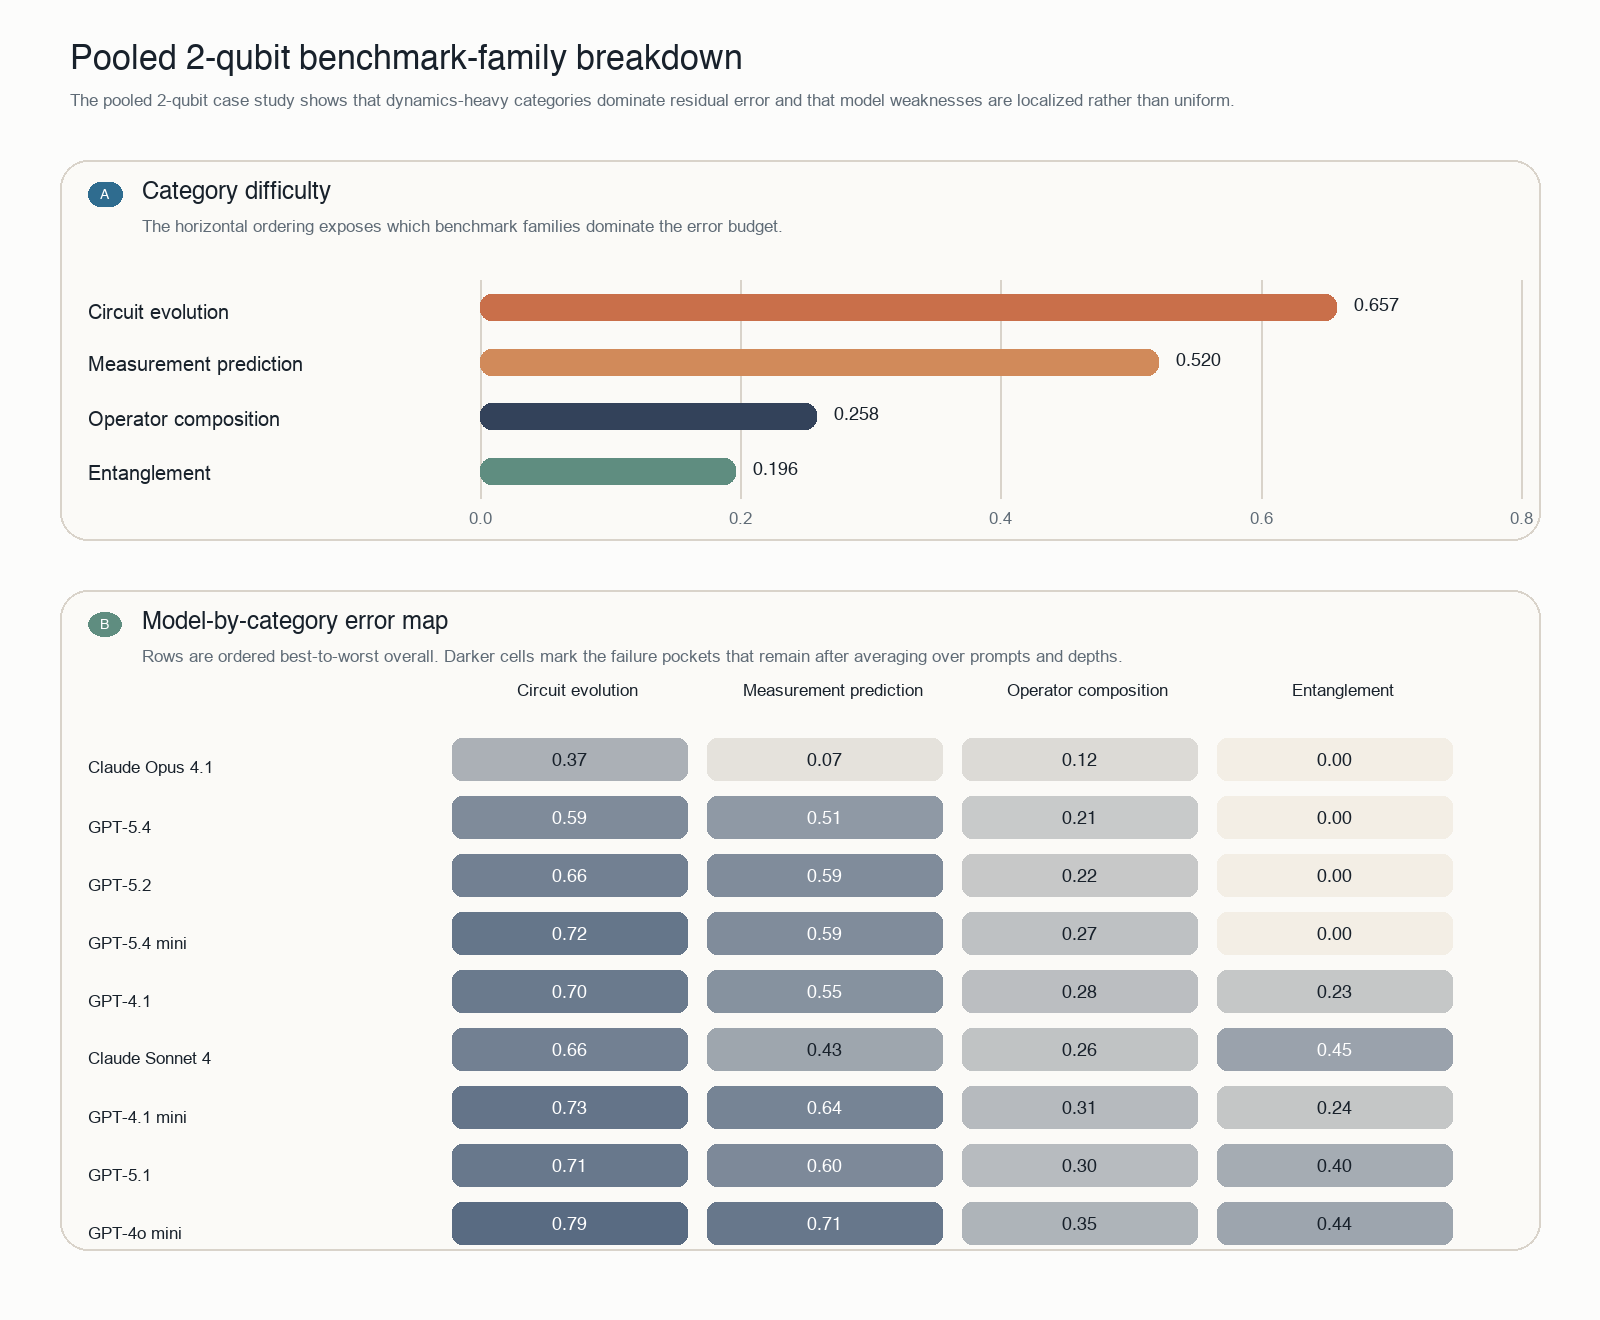
\includegraphics[width=0.96\linewidth]{../artifacts/figures/combined_quantum_breakdown.png}
\caption{Benchmark-family breakdown in the pooled case study. Left: overall category difficulty. Right: model-by-category heatmap showing where each model fails most strongly.}
\label{fig:breakdown}
\end{figure}

\subsection{4-qubit stress test}
The matched 4-qubit stress test shows that benchmark difficulty rises substantially once the state space is enlarged. Across the same GPT and Claude model sets, overall mean normalized error increases from 0.408 on the 2-qubit benchmark to 0.533 on the 4-qubit benchmark, a delta of $+0.125$. If we restrict attention to the three categories that actually scale from 2 to 4 qubits, the increase is larger: GPT models rise by $+0.166$ on average, and Claude models rise by $+0.192$.

The degradation is concentrated in the same places that were already hardest in the main benchmark. In the pooled 2q$\rightarrow$4q comparison, circuit evolution increases by $+0.185$ and measurement prediction by $+0.188$. Entanglement classification also worsens by $+0.142$, while operator composition changes by $-0.013$ because it is intentionally held fixed as a one-qubit control task rather than scaled to a 16$\times$16 matrix-return problem. This makes the 4-qubit result easier to interpret: the observed degradation is not a generic artifact of longer prompts alone, but a difficulty increase in the genuinely state-space-sensitive parts of the benchmark.

The family-level pattern is consistent across providers. For GPT models, mean error rises from 0.440 to 0.561. For Claude models, mean error rises from 0.294 to 0.437. The strongest individual models remain the strongest under the stress test, but they still lose ground. Claude Opus 4.1 rises from 0.138 to 0.298, and \texttt{gpt-5.4} rises from 0.329 to 0.525. The stress test therefore supports a stronger claim than the original 2-qubit benchmark alone: current models are not only imperfect on elementary quantum tasks, but they degrade materially as the underlying Hilbert space grows.

\begin{figure}[tbp]
\centering
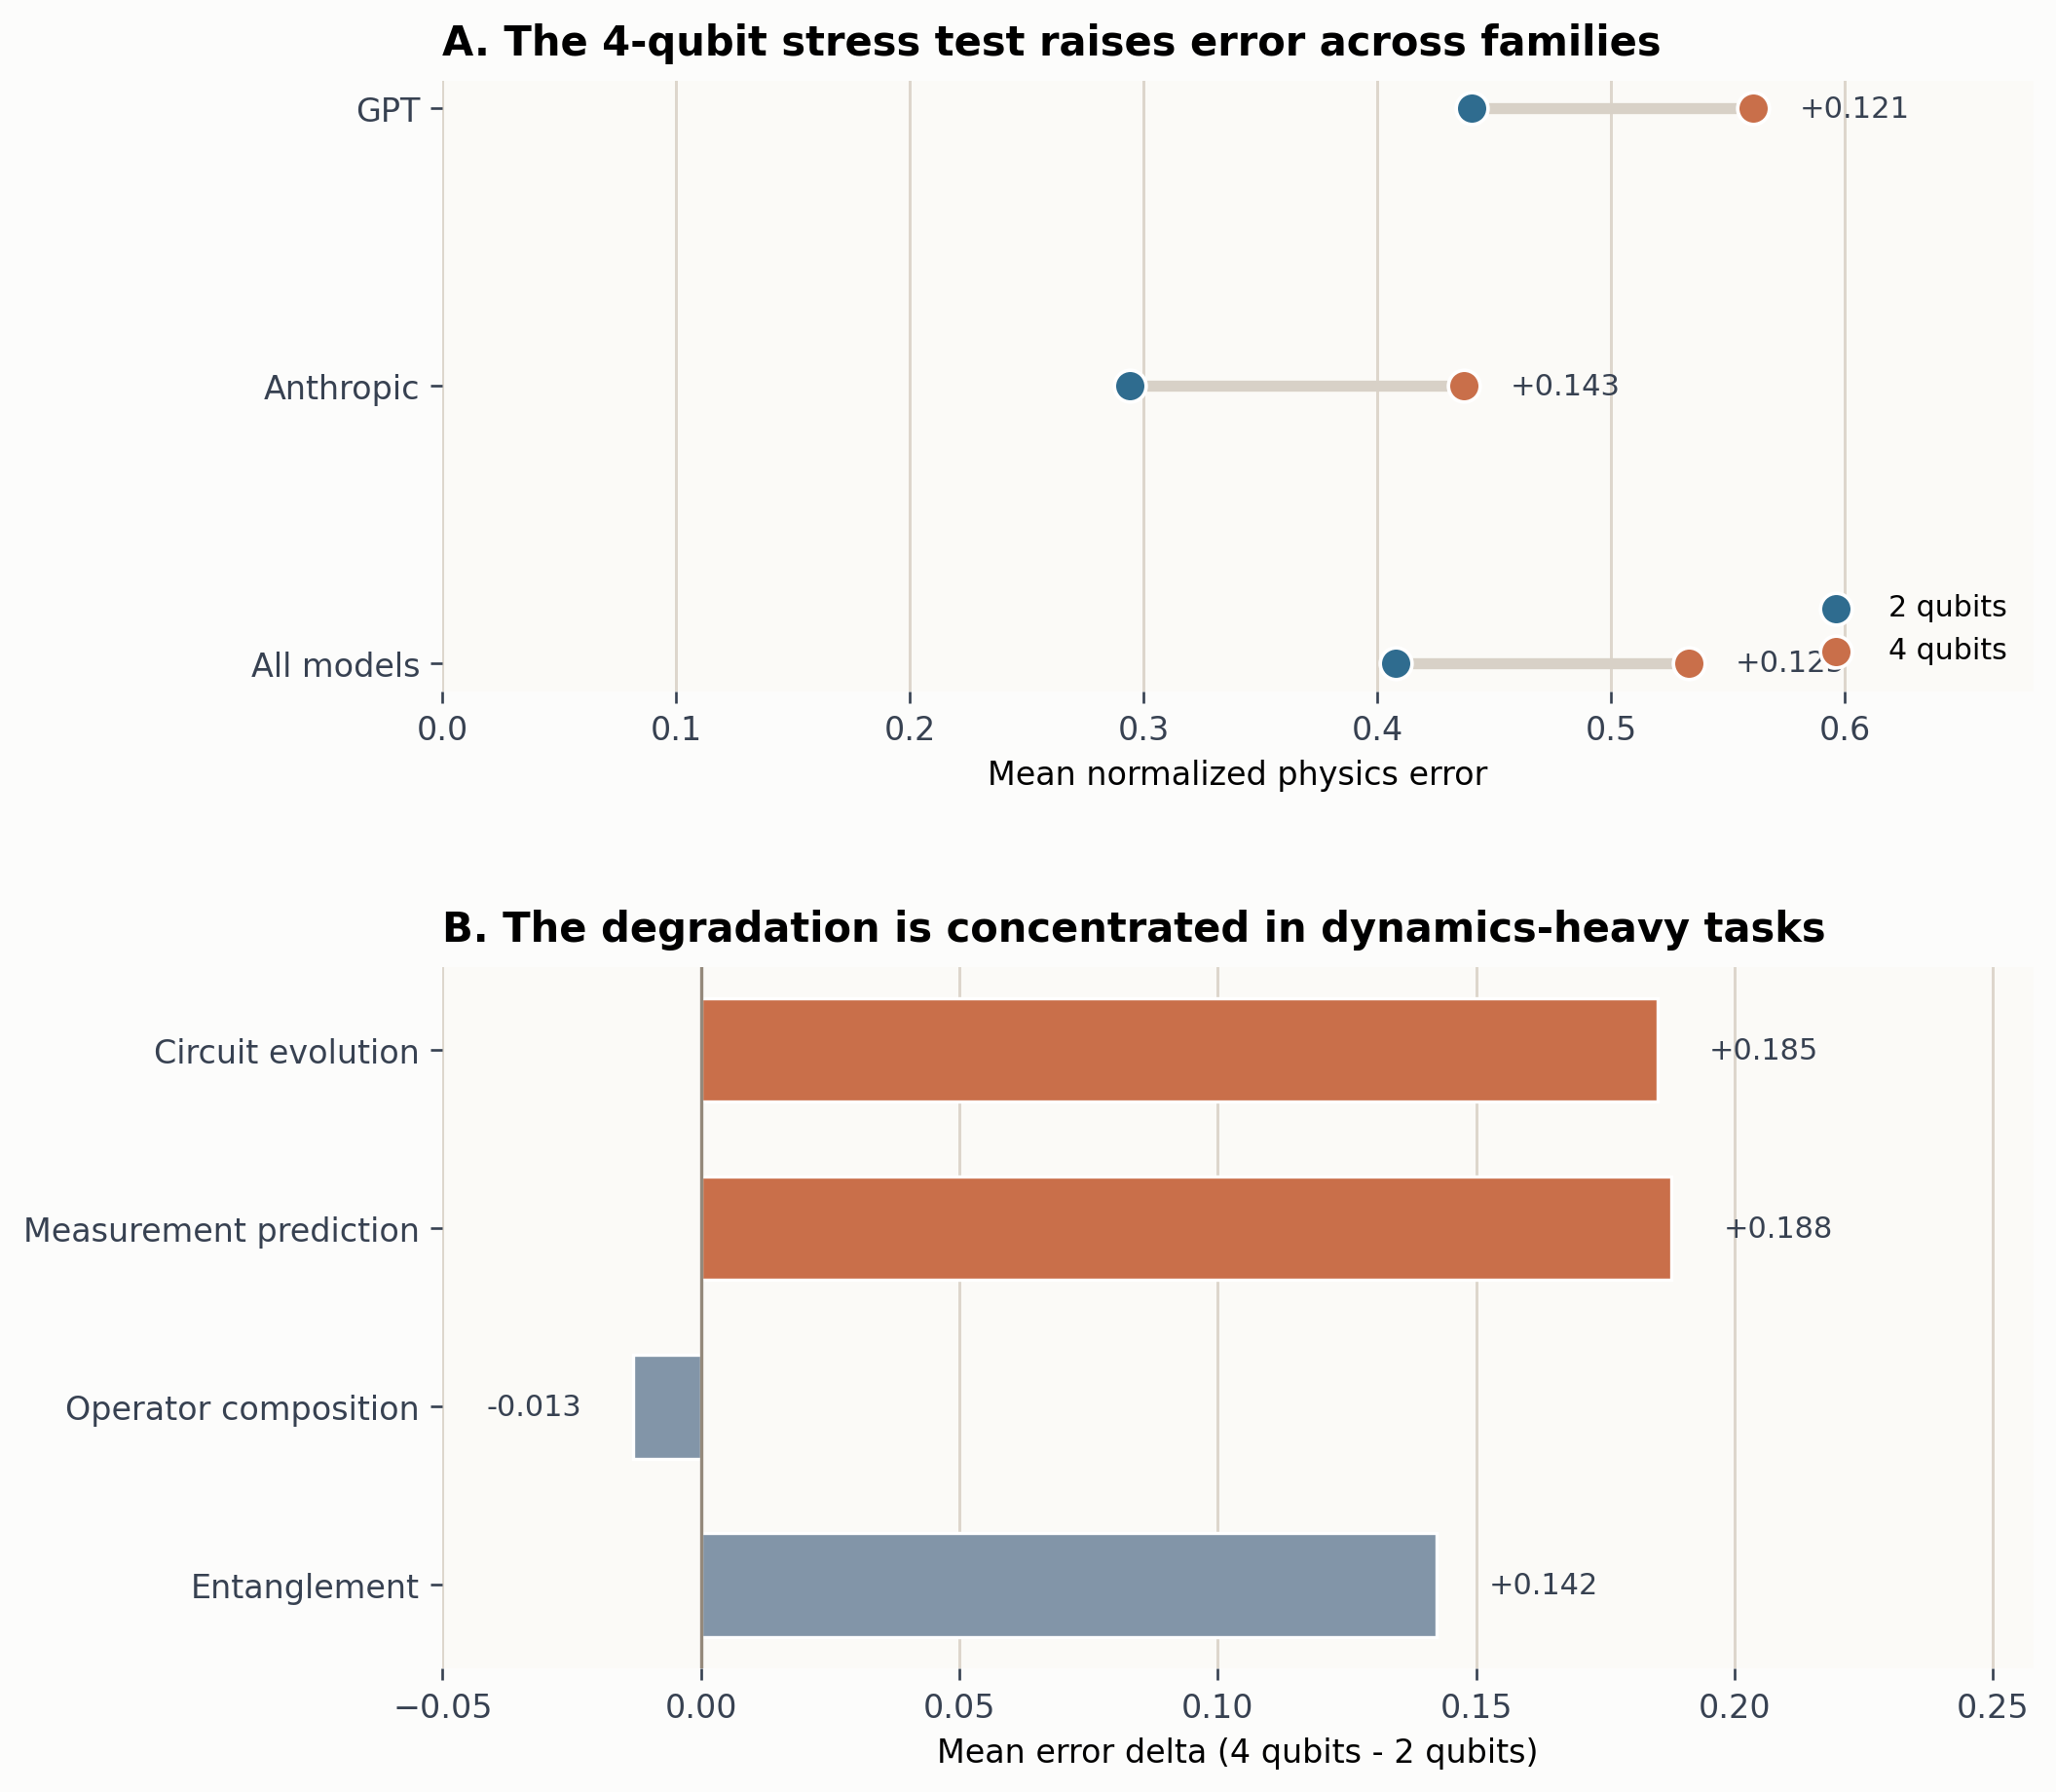
\includegraphics[width=0.98\linewidth]{../artifacts/figures/qubit_stress_test.png}
\caption{Matched 2-qubit versus 4-qubit stress test. Left: both GPT and Claude families get worse when the benchmark is rerun at 4 qubits. Right: the largest degradations occur in circuit evolution and measurement prediction, while the unchanged operator-composition control slice remains nearly flat.}
\label{fig:qubit-stress}
\end{figure}

\subsection{Ablations}
Additional ablations sharpen the main picture. First, the depth manipulation is weak not only in aggregate but also within individual models: most model-specific depth curves are nearly flat, and where differences do exist they are small relative to cross-model gaps. Second, the stronger GPT-5 and Claude 4 models improve over the weaker GPT-4-family slice in every benchmark category, with the largest gains appearing outside circuit evolution. Third, stronger models are not simply converting catastrophic failures into milder failures; they also increase exact-correct rates while reducing full-error failures.

\subsubsection{Time-budget repair and feedback}
The repair ablation adds a more operational view of the benchmark. As shown in Table~\ref{tab:feedback-overall}, repeated attempts help substantially, but verifier-guided retry helps more than blind self-retry. Solved fraction rises from 0.422 in the one-shot condition to 0.609 under self-retry and 0.688 under verifier feedback. Verifier feedback is also slightly more efficient on solved prompts: its mean solve time is 2.350\,s versus 2.650\,s for self-retry, and its median solve time is 1.025\,s versus 1.288\,s.

\begin{table}[t]
\centering
\caption{Feedback ablation on a strong-model subset under a 5-minute per-prompt budget. The subset contains 64 tasks total, depth 4 only.}
\label{tab:feedback-overall}
\begin{tabular}{lrrr}
\toprule
Mode & Solve rate & Mean solve time (s) & Median solve time (s) \\
\midrule
One-shot & 0.422 & 0.835 & 0.732 \\
Self-retry & 0.609 & 2.650 & 1.288 \\
Verifier feedback & 0.688 & 2.350 & 1.025 \\
\bottomrule
\end{tabular}
\end{table}

The gain is not uniform across task families. Under the same 64-task subset, circuit evolution improves from 0.250 solved fraction in the one-shot setting to 0.500 with verifier feedback; measurement prediction improves from 0.250 to 0.562; and operator composition improves from 0.250 to 0.688. Entanglement classification is already nearly saturated in the one-shot condition (0.938) and reaches 1.000 under verifier feedback. These category-level improvements show that some hard failures are repairable, but they also preserve the same ordering seen in the main benchmark: the dynamics-heavy tasks remain the limiting cases.

\begin{figure}[tbp]
\centering
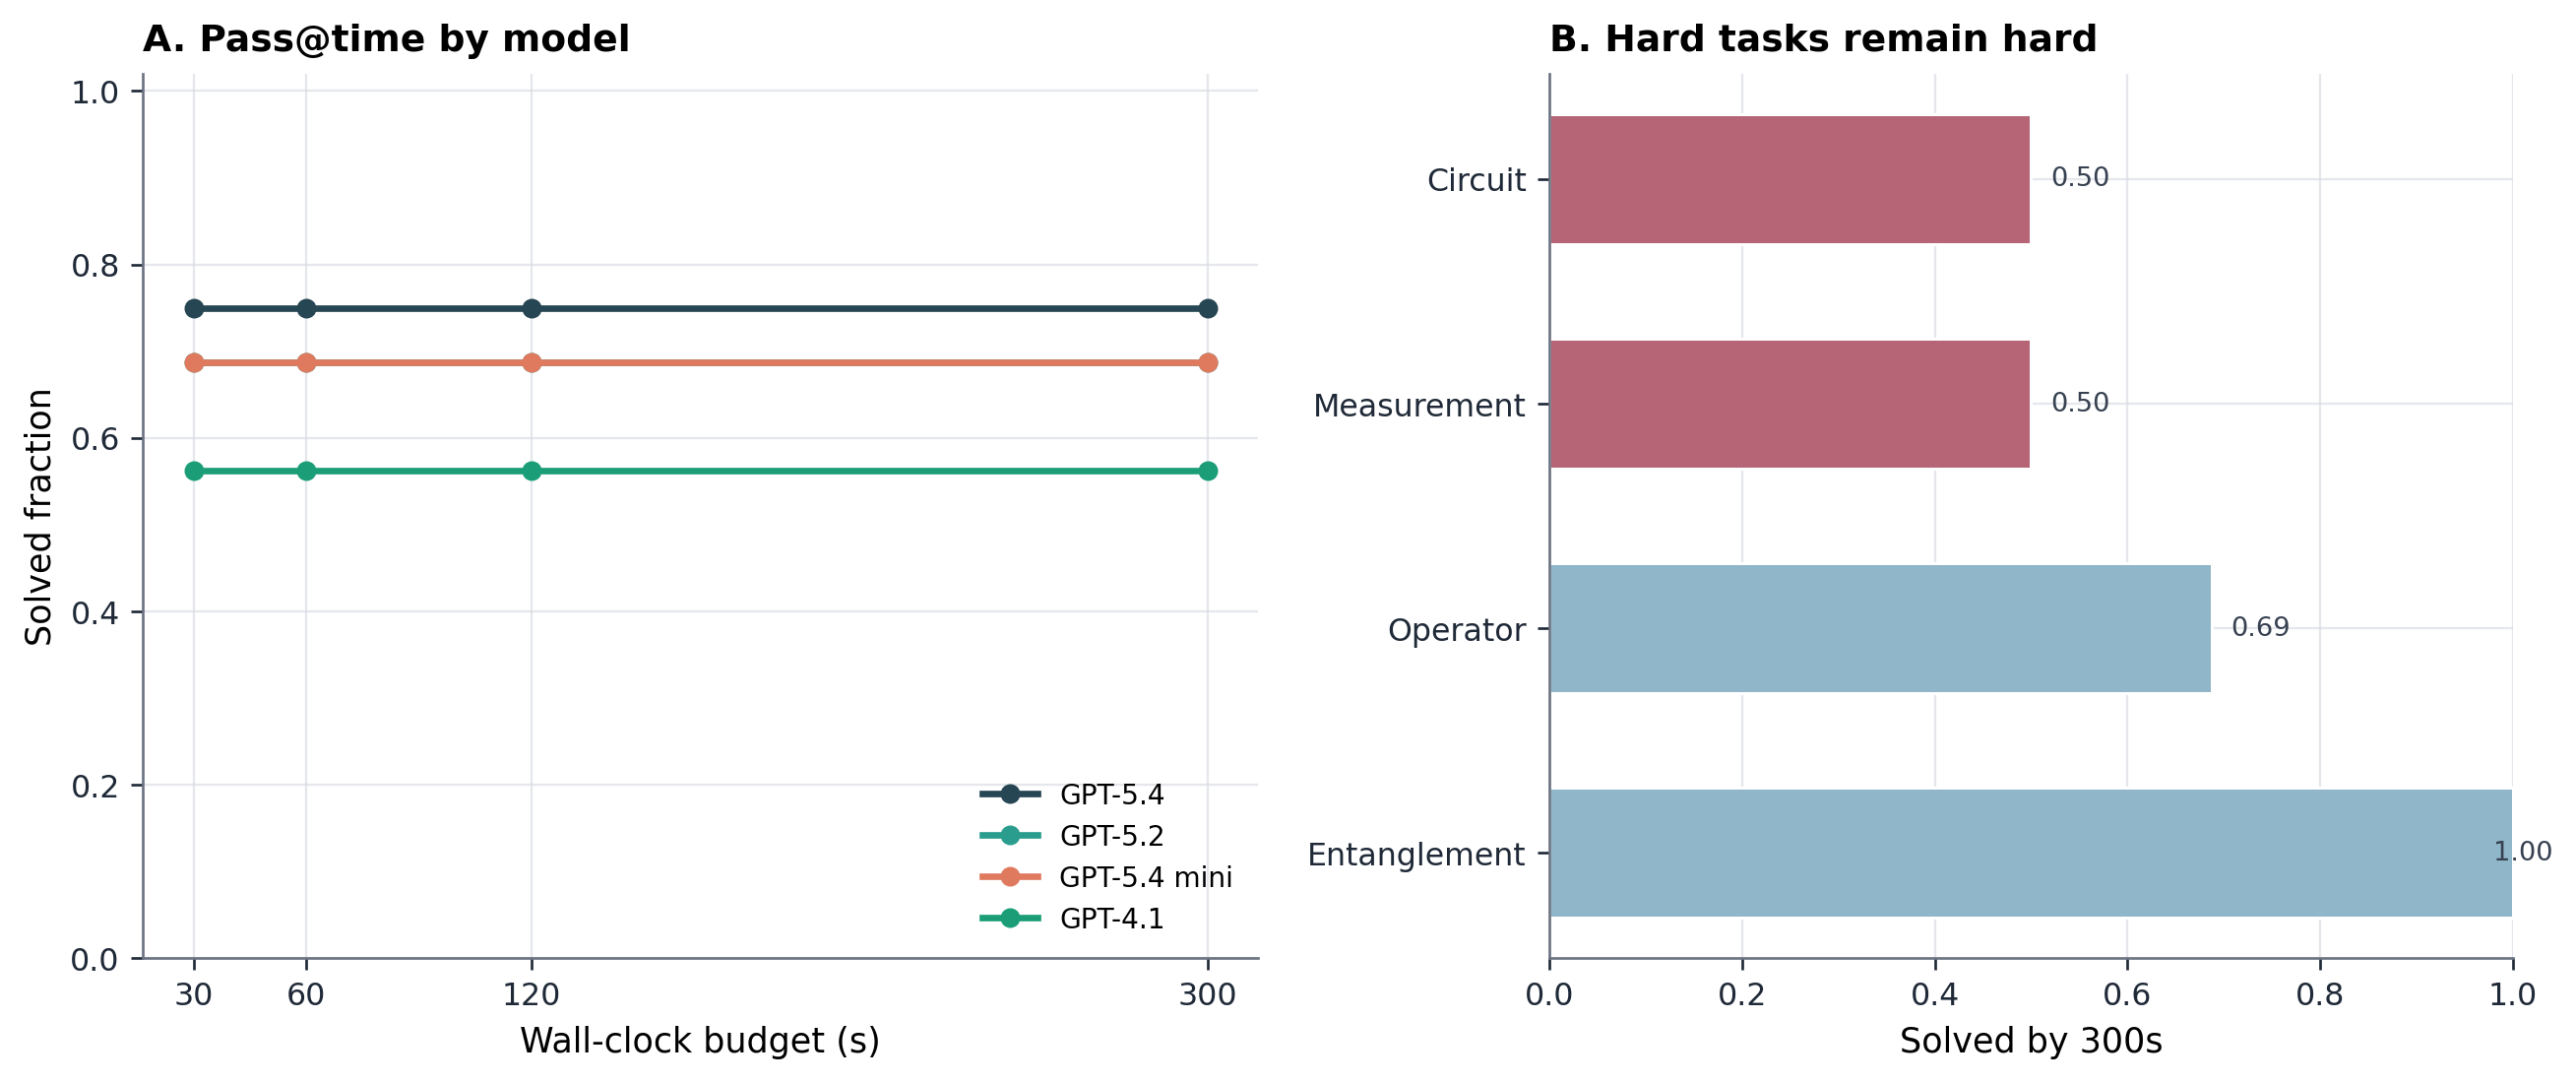
\includegraphics[width=0.96\linewidth]{../artifacts/figures/timebudget_strong_models_progress.png}
\caption{Verifier-feedback time-budget run on the strong-model subset. Left: solved fraction by wall-clock budget for each model. Right: solved fraction by category under the full 300-second budget. In practice the curves plateau early: pass@30s, pass@60s, pass@120s, and pass@300s are identical at 0.688 overall.}
\label{fig:timebudget}
\end{figure}

Figure~\ref{fig:timebudget} makes the key point visible: nearly all recoverable gains happen very early. In the verifier-feedback run, pass@30s, pass@60s, pass@120s, and pass@300s are all equal to 0.688. This means the remaining failures are not being rescued by simply allowing more wall-clock time. The evidence therefore suggests a mixed picture: iterative repair helps, explicit feedback helps more, but extra time alone does not solve the core quantum-dynamics failure modes.

We observe the same qualitative pattern on the Claude subset once output extraction is made robust to mixed prose and code-block responses. On a matched 32-task Anthropic subset using Claude Sonnet 4 and Claude Opus 4.1, solve rate rises from 0.594 in the one-shot condition to 0.813 under self-retry and 0.938 under verifier feedback. The gain is concentrated in Claude Sonnet 4, which improves from 0.188 to 0.625 to 0.875 across the three modes, while Claude Opus 4.1 solves the subset in every mode. This suggests that the repair result is not specific to one provider family, but that output-format robustness in the evaluator matters for fair cross-provider comparisons.

\section{Discussion}
The case study supports five practical conclusions.

First, quantum hallucination is measurable in a fully automated setting. Many outputs are syntactically clean and machine-readable, yet remain physically wrong under exact evaluation. This makes the benchmark useful as a reliability diagnostic rather than merely as a formatting test.

Second, model capability matters more than prompted depth in the present setup. The strongest result is the pooled capability trend; the depth manipulation is small relative to that effect and does not separate from zero under bootstrap uncertainty.

Third, some failures are recoverable under iterative interaction, but the mechanism matters. Blind self-retry improves solve rate over a one-shot baseline, while verifier-guided retry improves it further, and this pattern appears in both the OpenAI and Anthropic repair subsets. At the same time, the time-budget curves flatten quickly, which indicates that the remaining hard cases are not simply waiting for more deliberation time.

Fourth, the benchmark identifies a concrete residual weakness: exact quantum state and probability evolution. This is more informative than a generic claim that models are unreliable on quantum tasks, because it isolates the specific computational burden that remains difficult even for stronger models.

Fifth, the new 4-qubit stress test shows that these failures do not remain confined to the easiest possible small systems. When we enlarge the state space while keeping the evaluation procedure matched, both GPT and Claude families degrade materially, and the degradation is concentrated in the same dynamics-heavy categories.

\section{Limitations}
QuantumPhysEval is intentionally narrow. It uses controlled small-system settings to enable exact scoring, but that also limits ecological breadth. Even with the added 4-qubit stress test, the benchmark remains far from realistic chemistry, control, or error-correction workloads. The model-size variable is a manually assigned proxy rather than a verified parameter count, and the pooled fit mixes families and release generations. The benchmark also uses a single prompt style per task family and a single temperature setting. The 4-qubit stress test does not upscale operator composition, since returning exact 16$\times$16 matrices would mostly measure formatting burden rather than useful reasoning. The repair ablation is smaller than the pooled study and uses a binary verifier signal that would not always be available in practical deployments. The present evidence therefore supports a strong benchmark-level capability trend, but it should not be overinterpreted as a universal scaling law.

\section{Conclusion}
In this paper, we introduced QuantumPhysEval, a benchmark for measuring quantum hallucinations as physics-grounded error on elementary quantum tasks. In a pooled 2-qubit case study over OpenAI GPT and Anthropic Claude models, benchmark error decreases strongly with model capability, while prompted reasoning depth shows no robust independent effect. A matched 4-qubit stress test shows that performance worsens materially once the state space expands, especially on circuit evolution and measurement prediction. Separate repair ablations show that repeated attempts can recover some failures, especially when verifier feedback is available, but those gains saturate quickly and do not erase the main weakness. These results suggest that language models can produce plausible quantum answers, but exact physical reliability remains limited and should be measured explicitly rather than assumed.

\appendix
\section*{Appendix: Live Statistical Snapshot}
\appendixsnapshot

\end{document}
